\documentclass[svgnames,tikz]{standalone}

\usepackage{newtxmath,libertine,anyfontsize,cancel}
\usetikzlibrary{tikzmark}
\tikzset
  {
    every node/.style =
      { align = center, DarkSlateGray!30, font = \footnotesize },
    every path/.style = { DarkSlateGray!30, line cap = round }
  }

\begin{document}
  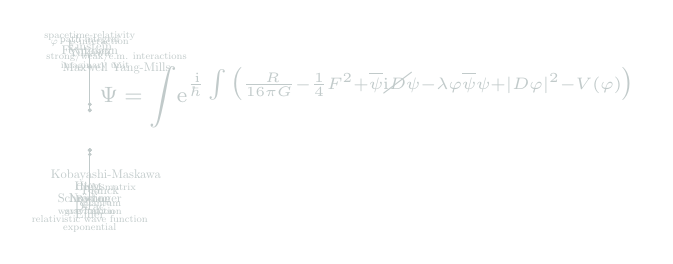
\begin{tikzpicture}
    \node [ above right ] at (0,0)
      {$\displaystyle
        \tikzmarknode a\Psi = \tikzmarknode b\int
        \tikzmarknode c{\mathrm e}^
          {
            \frac{\tikzmarknode d{\mathrm i}}{\tikzmarknode e\hbar}
            \int\big(
              \frac{\tikzmarknode fR}{16\pi \tikzmarknode gG}-
              \frac14\tikzmarknode hF^2+
              \overline\psi\mathrm i\tikzmarknode i{\cancel D}\psi-
              \tikzmarknode j\lambda
              \tikzmarknode k{\varphi\overline\psi}\psi+
              |D\tikzmarknode l\varphi|^2-V(\varphi)
            \big)
          }
      $};
    \draw ([yshift = -1ex]a.south) coordinate (A) --++ (0,-.5)
     node [ scale = .45, below ]
      { \normalsize Schr\"odinger\\ wave function};
    \draw ([yshift = 1ex]b.north) coordinate (B) --++ (0,.55)
     node [ scale = .45, above ] { path integral\\\normalsize Feynmann };
    \draw ([yshift = -1ex]c.south) coordinate (C) --++ (0,-.7)
     node [ scale = .45, below] { \normalsize  Euler\\ exponential};
    \draw ([yshift = 1ex]d.north) coordinate (D) --++ (0,.45)
     node [ scale = .45, above, xshift = 1ex] { imaginary unit};
    \draw ([yshift = -1ex]e.south) coordinate (E) --++ (0,-.4)
     node [ scale = .45, below, xshift = 2ex]
      { \normalsize Planck\\ quantum};
    \draw ([yshift = 1ex]f.north) coordinate (F) --++ (0,.7)
     node [ scale = .45, above ]
      { spacetime-relativity\\\normalsize Einstein};
    \draw ([yshift = -1ex]g.south) coordinate (G) --++ (0,-.5)
     node [ scale = .45, below ] { \normalsize Newton\\ gravitation};
    \draw ([yshift = 1ex]h.north) coordinate (H) --++ (0,.4)
     node [ scale = .45, above, xshift = 5ex ]
      { strong/weak/e.m. interactions\\\normalsize Maxwell Yang-Mills};
    \draw ([yshift = -1ex] i.south) coordinate (I) --++ (0,-.6)
     node [ scale = .45, below ]
      { \normalsize Dirac\\ relativistic wave function};
    \draw ([yshift = -1ex] j.south) coordinate (J) --++ (0,-.2)
     node [ scale = .45, below, xshift = 3ex]
      { \normalsize Kobayashi-Maskawa\\ CKM matrix };
    \draw ([yshift = 1ex] k.north) coordinate (K) --++ (0,.55)
     node [ scale = .45, above ]
      { $\varphi$ - $\psi$ interaction\\\normalsize Yukawa};
    \draw ([yshift = -1ex] l.south) coordinate (L) --++ (0,-.3)
     node [ scale = .45, below ] { \normalsize Higgs\\ Boson};
    \foreach \x in {A,B,...,L}
      \fill [ DarkSlateGray!30 ] (\x) circle (.025);
  \end{tikzpicture}
\end{document}
